\documentclass[aspectratio=169,11pt]{beamer}
% Aspect ratio:
% 610 => 16:10 
% 169 => 16:9 (Mas común actualmente)
% 149 => 14:9
%  54 => 5:4
%  43 => 4:3 (Default)
%  32 => 3:2

% Tamaño de la fuente
% 8pt, 9pt, 10pt, 11pt (default), 12pt, 14pt, 17pt, 20pt

% Opciones de lenguaje usando polyglossia (defino dos para este documento)
\usepackage{polyglossia}
\setmainlanguage{spanish}
\setotherlanguage[variant=american]{english}

\usepackage{anyfontsize}

% Los símbolos el los conjuntos numéricos
\usepackage{amssymb} 

 % Incluir imágenes
\usepackage{graphicx}
% Poder usar subfiguras
\usepackage{subcaption} 
% Para presentaciones usualmente no necesitamos la primer parte del caption
\captionsetup[figure]{labelformat=empty}
\captionsetup[subfigure]{labelformat=empty}
%\captionsetup[table]{labelformat=empty}

% Tablas con estilo profesional
\usepackage{booktabs}

% Para usar varias columnas
\usepackage{multicol}

% Para usar las comillas en español
\usepackage{dirtytalk}

% Crear un comando para el email
\newcommand{\email}[1]{
    \texttt{
      \href{mailto:#1}{#1}
    }
}

% Construyendo la diapositiva de titulo
\title[La torre del elefante]{La torre del elefante}
\subtitle{de Robert E. Howard}
\author[Nemediano]{Análisis de una historia de Conan por Nemediano}
\institute[El baúl de Howard]{
%     email for contact
    \normalsize{\email{https://nemediano.github.io/canalREH/}}
%    university name
%    \unam
}
\date{}
%\date[Noviembre 2023] % (optional)
%{Congreso Nacional de Software Libre, Abril 2021}
%\titlegraphic{\includegraphics[width=1.7cm]{img/escudo-a}}

% Para que el logo parezca en todas las diapositivas
%\logo{\includegraphics[height=1cm]{img/escudo-a}}

\usetheme{AnnArbor}
\useinnertheme{circles}
\usecolortheme{orchid}
% El tema Annharbor no usa comando de alerta. Los redefinimos
\setbeamercolor{block title alerted}{fg=white,bg=red}
\setbeamercolor{alerted text}{fg=red}

% Pongo linkcolor vacío para que los links internos no tengan color
% Solo los links externos tienen color
\hypersetup{colorlinks,linkcolor=,urlcolor=blue}

\setbeamertemplate{caption}{\insertcaption}
\beamertemplatenavigationsymbolsempty

\begin{document}

% El contenido de la presentación esta en este otro archivo
% Primer slide contiene el título
\begin{frame}{}
    \maketitle
\end{frame}

%Segundo slide el índice
\begin{frame}{Agenda}
    \tableofcontents
\end{frame}

\begin{frame}{La torre del elefante}
\begin{columns}
\column[t]{0.5\textwidth}
 \begin{figure}[htb]
  \centering
  \includegraphics[width=0.5\textwidth]{img/Intro}
\end{figure}    
\column[t]{0.5\textwidth}
     \begin{itemize}
         \item Una historia corta de Robert E. Howard
         \item Una de sus mejores historias
         \item Espada y hechizería pura
         \begin{itemize}
          \item Ilustración de Mark Schultz
         \end{itemize}
     \end{itemize}
\end{columns}
\end{frame}

\section{Introducción}
\subsection{Editorial}
\begin{frame}{Publicación}
\begin{columns}
\column[t]{0.4\textwidth}
    \begin{figure}[htb]
    \centering
        \includegraphics[width=0.5\textwidth]{img/WeirdTales-1933-03}
        \caption{Marzo de 1933}
    \end{figure}    
\column[t]{0.6\textwidth}
    \begin{itemize}
         \item Publicada por primera vez en Weird Tales
         \item Alrededor de unas 20 páginas.
         \begin{itemize}
            \item 9800 palabras en Ingles
            \item 10600 palabras en Español
            \item Lectura en 40-50 minutos
         \end{itemize}
         \item Una historia de su personaje mas famoso: Conan el bárbaro
         \item Muchas veces publicada en Español y en el idioma original
    \end{itemize}
\end{columns}
\end{frame}

\begin{frame}{Orden de publicación del ciclo de Conan}
\begin{figure}[htb]
  \centering
  \includegraphics[width=0.32\textwidth]{img/OrdenPublicacion}
\end{figure}
\end{frame}

\begin{frame}{Cronología ficticia del personaje}
\begin{figure}[htb]
  \centering
  \includegraphics[width=0.85\textwidth]{img/Cronollogias}
\end{figure}
\end{frame}

\begin{frame}{Espacio en la edad Hiboria}
\begin{figure}[htp]
 \centering
 \begin{subfigure}[b]{0.5\textwidth}
   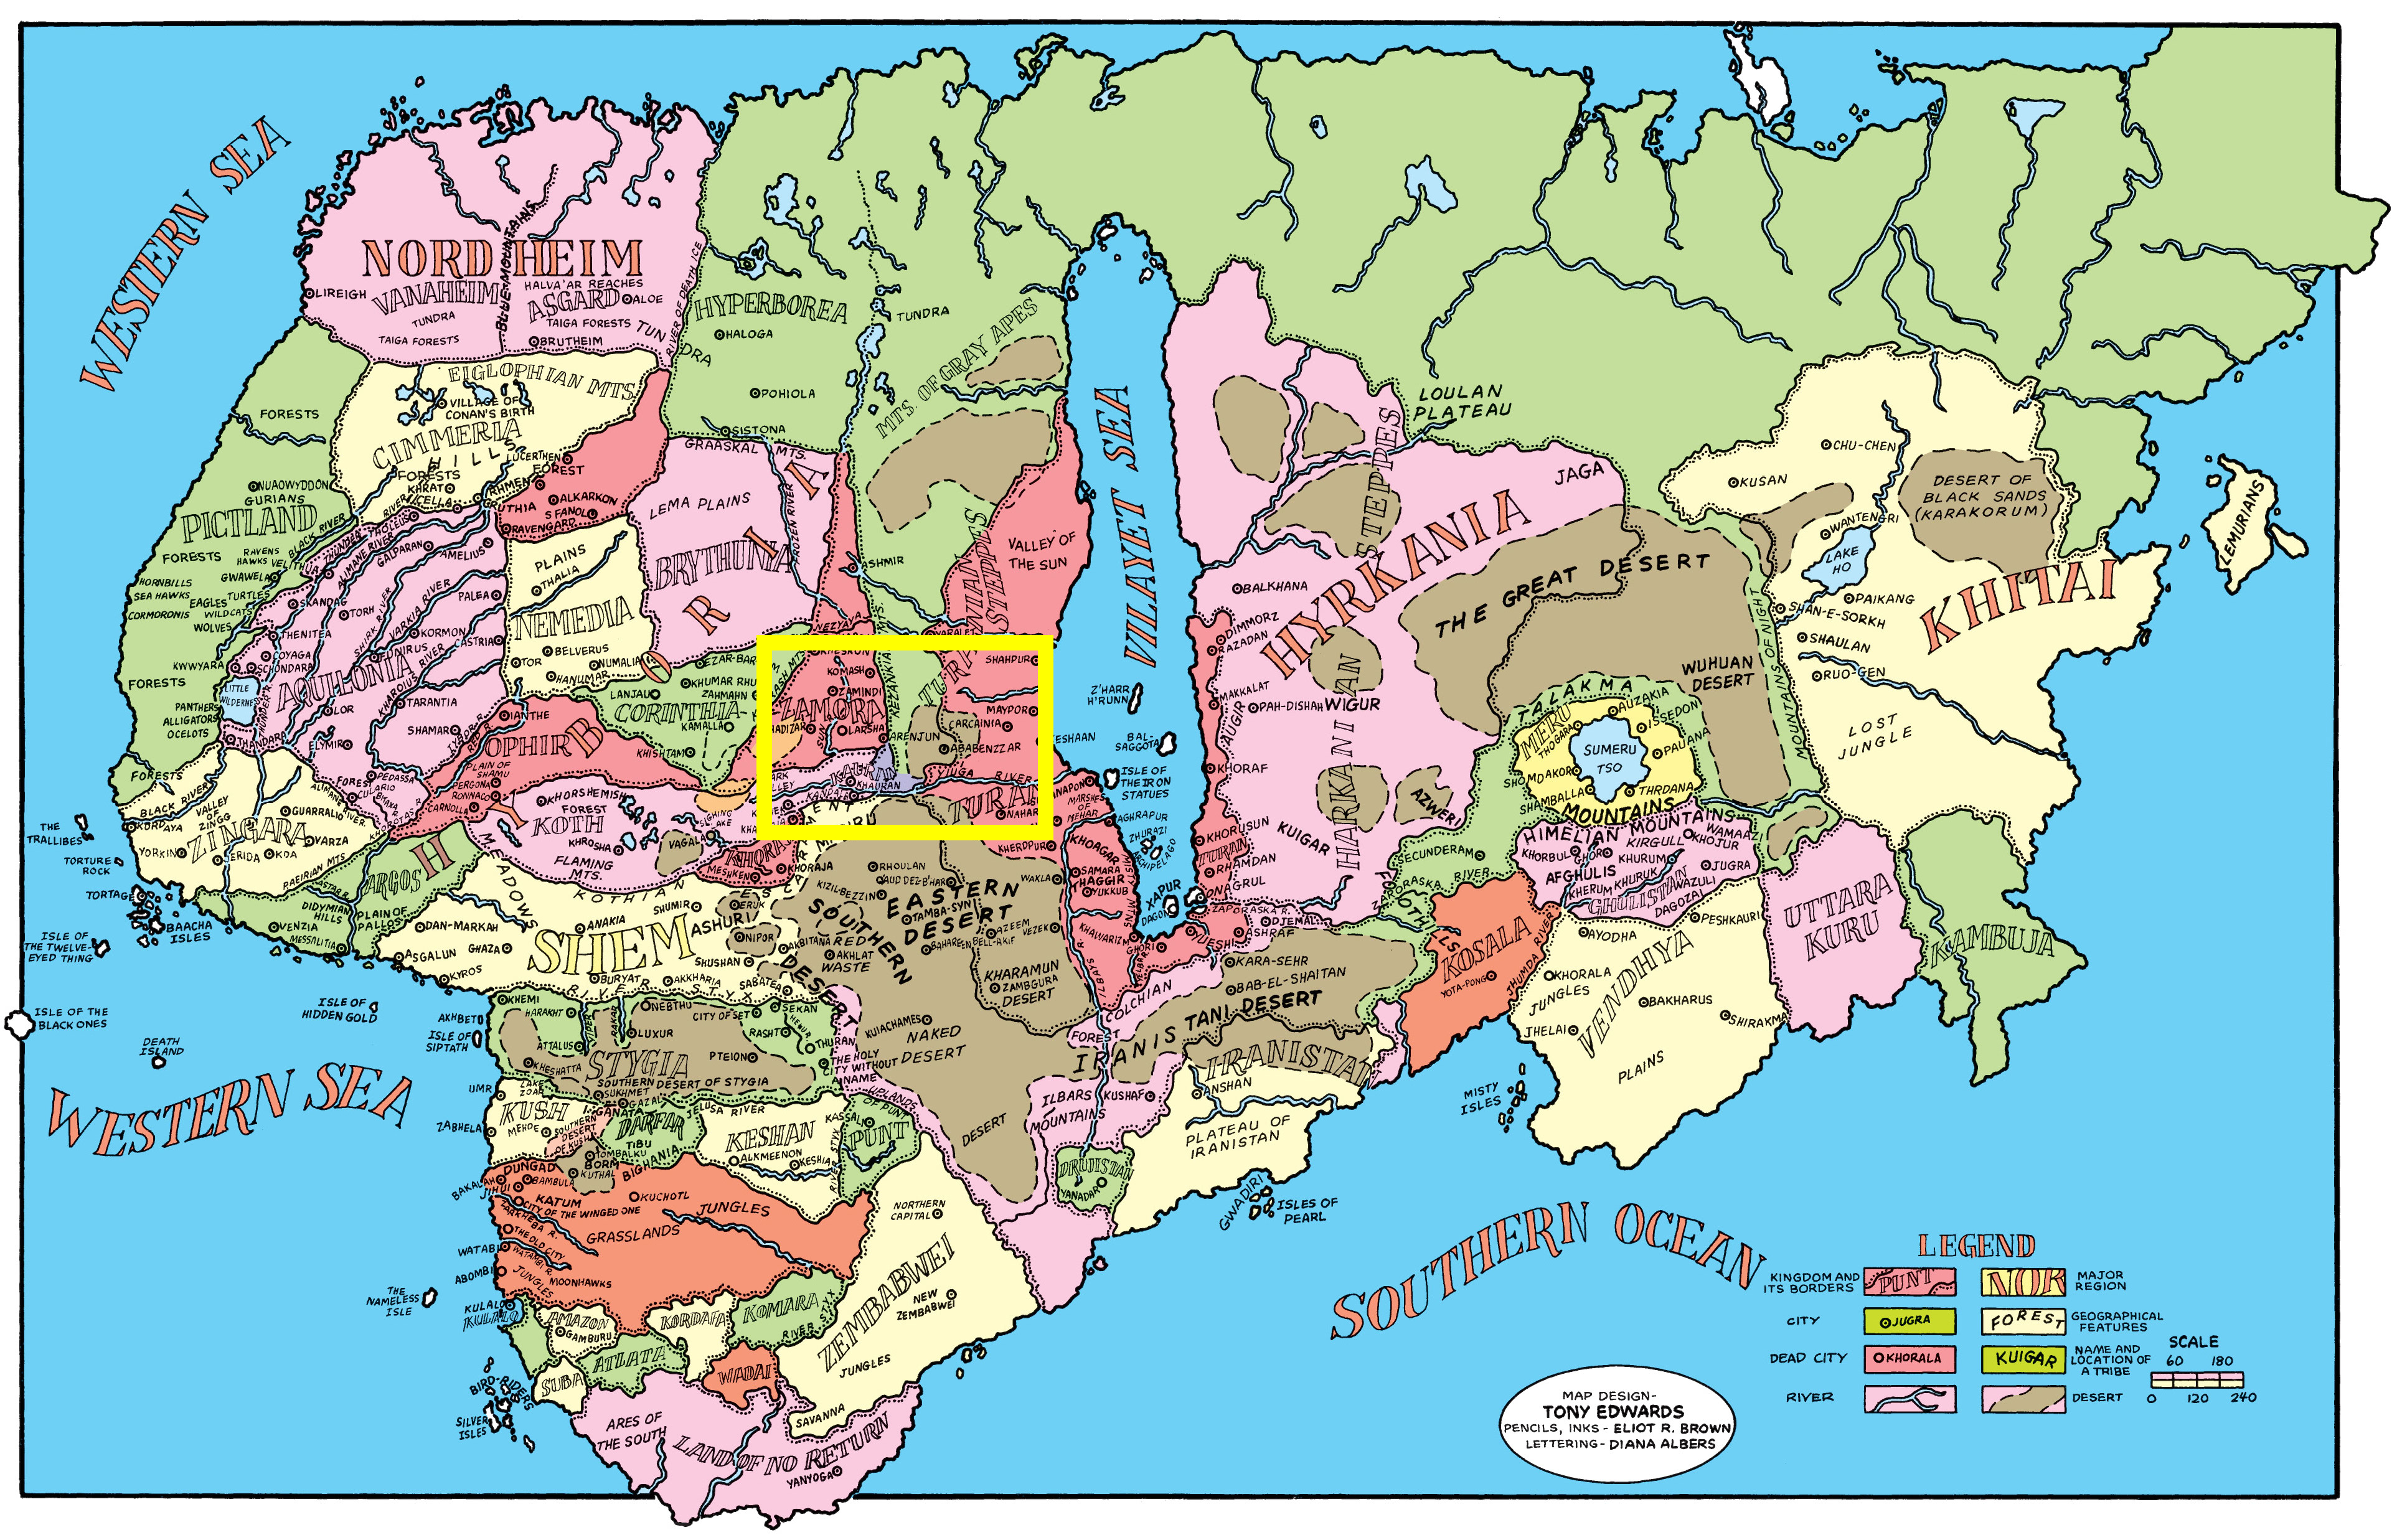
\includegraphics[width=\textwidth]{img/mapas/todo}
   %\caption{Barry Windsor Smith}
 \end{subfigure}
~
 \begin{subfigure}[b]{0.46\textwidth}
   \includegraphics[width=\textwidth]{img/mapas/inset}
   %\caption{Silvio \say{Sal} Buscema}
 \end{subfigure}
 \caption{La ciudad de Arenjun en la provincia de Zamora. La \say{ciudad de los ladrones}}
 \end{figure}
\end{frame}

\subsection{Adaptaciones}

\begin{frame}{Conan the barbarian}
\begin{columns}
\column[t]{0.4\textwidth}
    \begin{figure}[htb]
    \centering
        \includegraphics[width=0.55\textwidth]{img/TheBarbarian004Portada}
        \caption{26 de Enero de 1971}
    \end{figure}    
\column[t]{0.6\textwidth}
    \begin{itemize}
         \item Número 4 en la serie
         \item 21 páginas
         \item Créditos:
         \begin{description}
            \item[Dibujante:] Barry Windsor Smith
            \item[Entintador:] Silvio \say{Sal} Buscema
            \item[Escritor:] Roy Thomas
            \item[Letrista:] Sam Rosen
            \item[Editor:] Stand Lee
         \end{description}
    \end{itemize}
\end{columns}
\end{frame}

% \begin{frame}{}
% \begin{figure}[htp]
%  \centering
%  \begin{subfigure}[b]{0.16\textwidth}
%    \includegraphics[width=\textwidth]{img/artistas/BarryWindsorSmith}
%    \caption{Barry Windsor Smith}
%  \end{subfigure}
% ~
%  \begin{subfigure}[b]{0.16\textwidth}
%    \includegraphics[width=\textwidth]{img/artistas/SalBuscema}
%    \caption{Silvio \say{Sal} Buscema}
%  \end{subfigure}
%  ~
%  \begin{subfigure}[b]{0.16\textwidth}
%    \includegraphics[width=\textwidth]{img/artistas/RoyThomas}
%    \caption{Roy Thomas}
%  \end{subfigure}
% ~
%  \begin{subfigure}[b]{0.16\textwidth}
%    \includegraphics[width=\textwidth]{img/artistas/SamRosen1964}
%    \caption{Sam Rosen}
%  \end{subfigure}
% ~
%  \begin{subfigure}[b]{0.16\textwidth}
%    \includegraphics[width=\textwidth]{img/artistas/StanLee}
%    \caption{Stand Lee}
%  \end{subfigure}
% \end{figure}
% \end{frame}




\begin{frame}{Conan}
\begin{columns}
\column[t]{0.6\textwidth}
\begin{figure}[htp]
 \centering
 \begin{subfigure}[b]{0.3\textwidth}
   \includegraphics[width=\textwidth]{img/DarkHorse20Portada}
   \caption{Septiembre}
 \end{subfigure}
~
 \begin{subfigure}[b]{0.3\textwidth}
   \includegraphics[width=\textwidth]{img/DarkHorse21Portada}
   \caption{Octubre}
 \end{subfigure}
 ~
 \begin{subfigure}[b]{0.3\textwidth}
   \includegraphics[width=\textwidth]{img/DarkHorse22Portada}
   \caption{Noviembre}
 \end{subfigure}
\end{figure}
\begin{center}
2005    
\end{center}
\column[t]{0.4\textwidth}
    \begin{itemize}
         \item \say{Conan de Dark Horse}
         \item Números 20, 21 y 22 en la serie
         \item 23, 25 y 26 pp. en cada ejemplar
         \item 20, 22 y 23 de la historia
         \item Créditos:
         \begin{description}
            \item[Artista:] Cary Nord
            \item[Artista(6pp):] Michael Kaluta
            \item[Escritor:] Kurt Busiek
            \item[Colorista:] Dave Steward
            \item[Portada:] José Ladrönn
            \item[Letrista:] Richard Starkings
         \end{description}
    \end{itemize}
\end{columns}
\end{frame}


\section{Resumen}

\begin{frame}{}
\begin{columns}
\column[t]{0.5\textwidth}
    \begin{figure}[htb]
    \centering
        \includegraphics[width=0.9\textwidth]{img/res/01}
        \caption{El Maul}
    \end{figure}    
\column[t]{0.5\textwidth}
    \begin{figure}[htb]
    \centering
        \includegraphics[width=0.9\textwidth]{img/res/02}
        \caption{Una taberna}
    \end{figure}    
\end{columns}
\end{frame}

\section{Análisis}
\subsection{Personajes}
\begin{frame}{Conan}
\begin{columns}
\column[t]{0.4\textwidth}
\begin{itemize}
 \item Un joven bárbaro del norte
 \item Intrepido, impulsivo y desconfiado
 \item Poco acostumbrado a la civilización
 \item Primitivo, fuerte y rebelde
\end{itemize}
\column[t]{0.6\textwidth}
\begin{figure}[htp]
 \centering
 \begin{subfigure}[b]{0.3\textwidth}
   \includegraphics[width=\textwidth]{img/conan/CTB}
 \end{subfigure}
~
 \begin{subfigure}[b]{0.27\textwidth}
   \includegraphics[width=\textwidth]{img/conan/DH}
 \end{subfigure}
~
 \begin{subfigure}[b]{0.23\textwidth}
   \includegraphics[width=\textwidth]{img/conan/TSSC}
 \end{subfigure}
\end{figure}
\end{columns}
\end{frame}

\subsection{Citas interesantes}

\begin{frame}{}
\begin{exampleblock}{Conan reflexiona sobre religión}
Había estado muchas horas en cuclillas en los patios de los filósofos, escuchando los razonamientos y discusiones de teólogos y maestros, y se había ido de allí confuso y perplejo y con una sola idea clara: que estaban todos locos.
\end{exampleblock}
\say{\textit{He had squatted for hours in the courtyard of the philosophers, listening to the arguments of theologians and teachers, and come away in a haze of bewilderment, sure of only one thing, and that, that they were all touched in the head.}}
\end{frame}


\subsection{Tropes literarios}
\begin{frame}{Espada y hechizeria}
\begin{columns}
\column[t]{0.4\textwidth}
 \begin{itemize}
    \item Temporalidad: una sola noche
    \item Aventura circunstancial
    \item No genero un cambio
    \item La espada: la justicia; la hechicería: el mal
 \end{itemize}
 \column[t]{0.6\textwidth}
 \begin{figure}[htb]
    \centering
    \includegraphics[width=0.8\textwidth]{img/tributos/elephant07}
    \caption{Abe Papakhian}
 \end{figure} 
 \end{columns}
\end{frame}

\subsection{Influencias}
\begin{frame}{}
 \begin{columns}
\column[t]{0.4\textwidth}
 Hay referencias a este relato en muchos otros medios:
\begin{itemize}
 \item El juego MMORPG: \say{wizard101 online}
 \item La serie \say{Conan the adventurer}
 \item Conan RPG de Mongoose
 \item El videojuego Conan Exiles
\end{itemize}
\column[t]{0.6\textwidth}
\begin{figure}[htp]
 \centering
 \begin{subfigure}[b]{0.3\textwidth}
   \includegraphics[width=\textwidth]{img/otros/Conantheadventurerlogo}
 \end{subfigure}
~
 \begin{subfigure}[b]{0.3\textwidth}
   \includegraphics[width=\textwidth]{img/otros/RPGgame}
 \end{subfigure}
~ 
 \begin{subfigure}[b]{0.3\textwidth}
   \includegraphics[width=\textwidth]{img/otros/TowerHelephant}
 \end{subfigure}
\\
 \begin{subfigure}[b]{0.6\textwidth}
   \includegraphics[width=\textwidth]{img/otros/trofeo}
 \end{subfigure}
\end{figure}
\end{columns}
\end{frame}

\begin{frame}{Tributos de varios artistas}
\begin{figure}[htp]
 \centering
 \begin{subfigure}[b]{0.22\textwidth}
   \includegraphics[width=\textwidth]{img/tributos/elephant06}
   \caption{Dai Nguyen}
 \end{subfigure}
~
 \begin{subfigure}[b]{0.22\textwidth}
   \includegraphics[width=\textwidth]{img/tributos/elephant08}
   \caption{Spencer Sheahan}
 \end{subfigure}
~
 \begin{subfigure}[b]{0.22\textwidth}
   \includegraphics[width=\textwidth]{img/tributos/elephant03}
   \caption{Sanjulian}
 \end{subfigure}
~
 \begin{subfigure}[b]{0.22\textwidth}
   \includegraphics[width=\textwidth]{img/tributos/elephant04}
   \caption{Benito Gallego}
 \end{subfigure}
\end{figure}
\end{frame}

%El último slide es igual al primero: titulo y datos de contacto
\begin{frame}{}
    \maketitle
\end{frame}


\end{document}
